\documentclass[a4paper]{article}
\usepackage[affil-it]{authblk}
%\usepackage[backend=bibtex,style=numeric]{biblatex}
\usepackage{graphicx} % Required for inserting images
\usepackage{caption}

\usepackage{ctex}
\usepackage{epstopdf}
\usepackage{amsfonts,amssymb}
\usepackage{tikz}
\usetikzlibrary{chains}
\usepackage{listings}
\usepackage{xcolor}
\usepackage{float}
\usepackage{hyperref}
\usepackage{bookmark}
\usepackage{subfig}
\usepackage{listings,matlab-prettifier} % MATLAB 美化包
% \lstset{
%         style=Matlab-editor,
%         numbers      = left,
%         frame        = single,
% }
\usepackage{amsmath}
\usepackage{chngcntr}
\counterwithout{equation}{section}
\counterwithout{figure}{section}

\usepackage{geometry}
\geometry{margin=1.5cm, vmargin={0pt,1cm}}
\setlength{\topmargin}{-1cm}
\setlength{\paperheight}{29.7cm}
\setlength{\textheight}{25.3cm}


\begin{document}
% =================================================
\title{NA Theoretical homework \#4}

\author{陈澎 Chen Peng 3220103443
  \thanks{Email: \texttt{cpzju@zju.edu.cn}}}
\affil{Xinji 2201, Zhejiang University }


\date{\today}

\maketitle

% ============================================
\section*{I.}
$$
477=(111011101)_2=(1.11011101)_2\times2^8.
$$

\section*{II.}
$$
\frac{3}{5}=(0.10011001\ldots)_2=(1.00110011\ldots)_2\times 2^{-1}.
$$

\section*{III.}
We can induce that $x_R=(1+\beta^{1-p})\beta^e$ and $x_L=(\beta-\beta^{1-p})\beta^{e-1}$. Then 
$$
x_R-x=\beta^{1+e-p},\ x-x_L=\beta^{e-p}.
$$ 

So $x_R-x=\beta(x-x_L)$.

\section*{IV.}
From II, we have $$\frac{3}{5}=(1.00110011\ldots)_2\times 2^{-1}.$$

It can be induced that $x_L=(1.0011\ldots001)_2\times 2^{-1}$ and $x_R=(1.0011\ldots010)_2\times 2^{-1}$.

It can be calculated that $x-x_L=\frac{3}{5}\times 2^{-24}$ and $x_R-x=\frac{2}{5}\times 2^{-24}$.

So $\mathrm{fl}(x)=x_R=(1.0011\ldots010)_2\times 2^{-1}$ and relative roundoff error is 
$$
E_{\mathrm{rel}}=\lvert \frac{x_R-x}{x}\rvert=\frac{2}{3}\times 2^{-24}.
$$

\section*{V.}
Set $\mathrm{fl}(x)=x(1+\delta)$. There exists $x_L,x_R\in \mathcal{F}$ such that $x_L$ and  $x_R$ are adjacent.

When $x=x_L$ or $x=x_R$, we have $\mathrm{fl}(x)=x$ and $delta=0$.

Otherwise $x_L<x<x_R$, then definition 4.22 and lemma 4.23 yield
$$
  |\mathrm{fl}(x)-x|<|x_R-x_L|\leq\epsilon_M \min(|x_L|,|x_R|)<2^{-23}|x|.
$$

Hence $-2^{-23}|x|<\mathrm{fl}(x)-x<2^{-23}|x|$, which yields $|\delta|<2^{-23}$. 

So the unit roundoff is $2^{-23}$.

\section*{VI.}
As the Taylor extension shows: 
$$
1-\cos x=\frac{x^2}{2}+o(x^2)
$$

So 
$$
1-\cos x=(0.00001\ldots)_2.
$$

When transfroming it to normal form, it loses 5 bits of precision.

\section*{VII.}
\section*{VII-a.}
Use Taylor extension 
$$
1-\cos x=\frac{x^2}{2!}-\frac{x^4}{4!}+\frac{x^6}{6!}-\frac{x^8}{8!}+\cdots.
$$

\section*{VII-b.}
Use trigonometric identity 
$$
1-\cos x=2\sin^2\frac{x}{2}.
$$

\section*{VIII.}
\section*{VIII-a.}
We have
$$
C_f(x)=\lvert \dfrac{x\cdot\alpha(x-1)^{\alpha-1}}{(x-1)^{\alpha-1}}\rvert=\lvert \dfrac{x\alpha}{x-1}\rvert.
$$

$C_f(x)\rightarrow+\infty$ as $x\rightarrow 1$.

\section*{VIII-b.}
$$
C_f(x)=\lvert \dfrac{x\frac{1}{x}}{\ln x}\rvert=\lvert \dfrac{1}{\ln x}\rvert.
$$

$C_f(x)\rightarrow+\infty$ as $x\rightarrow 1$.

\section*{VIII-c.}
$$
C_f(x)=\lvert \dfrac{x e^x}{e^x}\rvert=\lvert x\rvert.
$$

$C_f(x)\rightarrow+\infty$ as $x\rightarrow \pm \infty$.

\section*{VIII-d.}
$$
C_f(x)=\lvert \dfrac{x \frac{-1}{\sqrt{1-x^2}}}{\arccos x}\rvert=\lvert \dfrac{x }{\sqrt{1-x^2} \arccos x}\rvert.
$$

$C_f(x)\rightarrow+\infty$ as $x\rightarrow \pm 1$.

\section*{IX.}
\section*{IX-a.}
For $x\in[0,1]$, we have 
$$
\begin{aligned}
  \mathrm{cond}_f(x)&=\lvert \frac{xf'(x)}{f(x)}\rvert\\
  &=\frac{xe^{-x}}{1-e^{-x}}\\
  &=\frac{x}{e^x-1}\\
  &\leq1.
\end{aligned}
$$

\section*{IX-b.}
$$
f_A=\mathrm{fl}[1-\mathrm{fl}(e^{-x})],
$$
which computes $f(x)=1-e^{-x}$ for $x\in[0,1]$.

$$
f_A=[1-e^{-x}(1+\delta_1)](1+\delta_2),
$$
where $|\delta_i\leq\epsilon_u$ for $i=1,2$.

Neglecting quadratic terms of $o(\delta_i^2)$, the above equation is equivalent to 
$$
f_A(x)=(1-e^{-x})(1+\delta_2-\frac{e^{-x}}{1-e^{-x}}\delta_1).
$$

Hence we have $\Phi(x)=1+\frac{e^{-x}}{1-e^{-x}}=\frac{1}{1-e^{-x}}$.

From theorem 4.78, we have 
$$
\mathrm{cond}_A(x)\leq \dfrac{\Phi(x)}{\mathrm{cond}_f(x)}\leq\frac{e^x}{x},
$$
for $x\in[0,1]$.

\section*{IX-c.}
As shown in Fig.$\ref{fig1}$, We can find that when $x$ is away form $0$, the value of $\mathrm{cond}_f(x)$ is small while $x$ is close to $0$, the estimate is quickly increasing and it is not practical.

\begin{figure}[H]
  \centering
  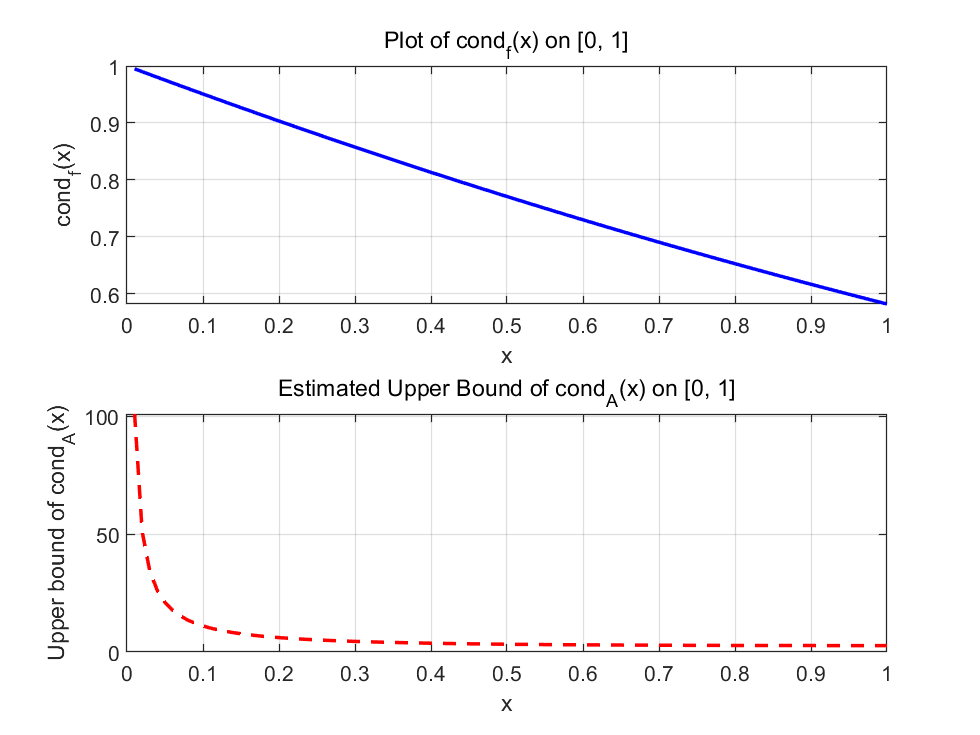
\includegraphics[width=0.6\textwidth]{./figure/IX-c.png}
  \renewcommand{\figurename}{Fig.}
  \caption{$\mathrm{cond}_A(x)$ and $\mathrm{cond}_f(x)$}
  \label{fig1}
\end{figure}

\section*{X.}
\section*{X-a.}
By singular value decomposition, we have $A=U\Sigma V$. So 
$$
\begin{aligned}
  \|A\|_2&=\|U\Sigma V\|_2=|\Sigma \|_2=\sigma_{\max}, \\
  \|A^{-1}\|_2&=\|V^{-1}\Sigma^{-1} U^{-1}\|_2\\
  &=\|V^{T}\Sigma^{-1} U^{T}\|_2\\
  &=\|\Sigma^{-1}\|_2\\
  &=\frac{1}{\sigma_{\min}}.
\end{aligned}
$$

So $\mathrm{cond}_2 A=\|A\|_2 \|A^{-1}\|_2=\frac{\sigma_{\max}}{\sigma_{\min}}.$

\section*{X-b.}
When $A$ is normal, by eigenvalue decomposition, we have $A=U\Sigma U^{T}$. Similarly it can be deduced that 
$$\begin{aligned}
  \|A\|_2&=|\lambda_{\max}|, \\
  \|A^{-1}\|_2&=|\frac{1}{\lambda_{\min}}|.
\end{aligned}$$

So $\mathrm{cond}_2 A=\|A\|_2 \|A^{-1}\|_2=\frac{\lambda_{\max}}{\lambda_{\min}}.$


\section*{X-c.}
When $A$ is unitary, it is clear that 
$$
\begin{aligned}
  \|A\|_2&=\|I_n\|=1, \\
  \|A^{-1}\|_2&=\|A^T\|_2=1.
\end{aligned}
$$

So $\mathrm{cond}_2 A=\|A\|_2 \|A^{-1}\|_2=1.$


\section*{XI.}
We have $q(r)$=0. So $\frac{\partial}{\partial a_i}q(r)=0$, for $i=0,1,\cdots,n-1$, i.e. 
$$
r^i+q'(r)\frac{\partial r}{\partial a_i}=0.
$$

Then 
$$
\frac{\partial r}{\partial a_i}=-\dfrac{r^i}{q'(r)}.
$$

Set $A(\mathbf{a})=[b_j(\mathbf{a})]_{1\times n}$, where $\mathbf{a}=[a_0,a_1,\ldots,a_{n-1}]^T$. From definition 4.71, we have 
$$
\begin{aligned}
  b_j(\mathbf{a})&=\lvert \dfrac{a_{j-1}\frac{\partial r}{\partial a_{j-1}}}{r} \rvert=\lvert \dfrac{r^{j-2}a_{j-1}}{q'(r)} \rvert,\\
  \mathrm{cond}_f(\mathbf{a})&=\|A(\mathbf{a})\|\\
  &=\max_{1\leq j\leq n}b_j(\mathbf{a})\\
  &=\max_{0\leq i\leq n-1}\lvert \dfrac{r^{i-1}a_{i}}{q'(r)} \rvert.
\end{aligned}
$$

For Wilkinson example, $p(x)=\prod_{k=1}^{p}(x-k)$, consider root $t\in\{1,2,\ldots,p\}$. So 
$$
\mathrm{cond}_f(\mathbf{a})=\max_{0\leq i \leq n-1} \frac{t^{i-1}|a_i|}{(t-1)!(p-t)!}
$$

The $mathrm{cond}_f(\mathbf{a})$ is nearly increasing with degree $i$, which means the conditional number can be huge.


\section*{XII.}



\section*{XIII.}
The width after $n$ iterations is $2^{-n}$. Let $2^{-n}<10^{-6}$, then $n\geq 20$.

Because $128=(10000000)_2$ and $129=(10000001)_2$, We can set the root as $r=M_0\times \beta^{e_0}$, $e_0=7$, $1\leq M_0 <2$. 

When $n\geq20$, $2^{-n}=2^{-n-7}\times 2^7$. We have $2^{-n-7}\leq 2^{-27}<2^{-23}=\epsilon_M$. So we can't compute the root with absolute accuracy $<10^{-6}$.


\section*{XIV.}
For $a=x_1<x_2<\cdots<x_N=b$, we construct a complete cubic spline and set $\mu_i=\frac{x_i-x_{i-1}}{x_{i+1}-x_{i-1}},\lambda_i=\frac{x_{i+1}-x_i}{x_{i+1}-x_{i-1}}$.From Theorem 3.7, We have 
$$\begin{bmatrix}2&\mu_{2}\\\lambda_{3}&2&\mu_{3}\\&&\ddots\\&&\lambda_{i}&2&\mu_{i}\\&&&\ddots&&\\&&&\lambda_{N-2}&2&\mu_{N-2}\\&&&&\lambda_{N-1}&2\end{bmatrix}\begin{bmatrix}m_{2}\\m_{2}\\\vdots\\m_{N-2}\\m_{N-1}\end{bmatrix}=\mathbf{b},$$
where $m_i = s'(f ; x_i)$ and the vector $\mathbf{b}$ is determined from the known information.

From Gershgorin Circle Theorem, we can estimate the eigenvalue of the matrix
$$
A=\begin{bmatrix}2&\mu_2&&&&&\\\lambda_3&2&\mu_3&&&&\\&&\ddots&&&&\\&&\lambda_i&2&\mu_i\\&&&&\ddots&&&\\&&&&\lambda_{N-2}&2&\mu_{N-2}\\&&&&&\lambda_{N-1}&2\end{bmatrix}.
$$

We have $$
|\lambda(A)-a_{ii}|\leq\sum_{j\neq i}|a_{ij}|,
$$
so $1\leq \lambda(A)\leq 3$.

So the condition number of the matrix $A$ is no more than 3. 

For uniform distribution spacing, the eigenvalue of A is $\lambda_k=2+\cos\frac{k\pi}{n-1},k=1,2,3,\cdots,n-2.$ The condition number is $\dfrac{2+\cos\frac{\pi}{n-1}}{2-\cos\frac{\pi}{n-1}}\approx3-\frac{2\pi^2}{(n-1)^2}+O\left(\frac1{(n-1)^4}\right)$.

But the extremely small spacing causes the difference quotient of certain elements in the right-hand vector $\mathbf{b}$ to become very large which means it is very sensitve. Besides, it causes smaller $\lambda_{\min}(A)$.

Thus one gets inaccurate results when the distance between two adjacent points is much smaller than those of other adjacent pairs. 



\section*{Exercise 4.33}
\section*{(a)}
(i)$b\leftarrow 8.769\times 10^4$; $e_c\leftarrow 4$.

(ii)$m_c\leftarrow 10.003$.

(iii)$m_c\leftarrow 1.0003$, $e_c\leftarrow 5$.

(iv)do nothing.

(v)$m_c\leftarrow 1.000$.

(vi)$c=1.000\times 10^5$.

\section*{(b)}
(i)$b\leftarrow -0.0005678\times 10^4$; $e_c\leftarrow 4$.

(ii)$m_c\leftarrow 1.2334322$.

(iii)do nothing.

(iv)do nothing.

(v)$m_c\leftarrow 1.233$.

(vi)$c=1.233\times 10^4$.

\section*{(c)}
(i)$b\leftarrow -0.5678\times 10^3$; $e_c\leftarrow 4$.

(ii)$m_c\leftarrow 0.6662$.

(iii)$m_c\leftarrow 6.662$, $e_c\leftarrow 3$.

(iv)do nothing.

(v)$m_c\leftarrow 6.662$.

(vi)$c=6.662\times 10^3$.

\section*{Exercise 4.42}
Set $p=2$, $\beta=10$, $a_1=4.9 \times 10^{-1}$, $a_2=1.0\times 10^1$, $a_3=4.2\times 10^0$, $a_4= 5.9\times 10^0$.

So $\text{fl}(a_1+a_2+a_3+a_4)=2.0\times 10^1$ and $\text{fl}(a_1+a_3+a_4+a_2)=2.1\times 10^1$ after sorting.

While $a_1+a_2+a_3+a_4=20.58$, we have $\delta_{\text{unsorted}}> \delta_{\text{sorted}}$ for this example.


\section*{Exercise 4.43}
\[
\text{fl}(a_1b_1 + a_2b_2 + a_3b_3) = \text{fl}\left( (a_1b_1) + (a_2b_2) + (a_3b_3) \right).
\]
For each product \( a_ib_i \), $i=1,2,3$, the rounding error is:
\[
fl(a_ib_i)=(1+\delta_i)a_i b_i, \quad |\delta|<\epsilon_u.
\]
Thus, from theorem 4.41, the total sum can be written as:
\[
\text{fl}(a_1b_1 + a_2b_2 + a_3b_3) = [a_1b_1(1+\delta_1) + a_2b_2(1+\delta_2) + a_3b_3(1+\delta_3)](1+\delta_0), \quad |\delta_0|<(1+\epsilon_u)^2-1\approx 2 \epsilon_u,
\]
i.e. 
$$
\text{fl}(a_1b_1 + a_2b_2 + a_3b_3)=(a_1b_1 + a_2b_2 + a_3b_3)(1+\delta), \quad |\delta|< 3\epsilon_u.
$$

Now, consider the case where we have multiple products and sums, such as:
\[
\text{fl}\left( \sum_{i=1}^{n} \prod_{j=1}^{m} a_{i,j} \right).
\]

Similarly, we have
$$
\text{fl}\left( \sum_{i=1}^{n} \prod_{j=1}^{m} a_{i,j} \right)=\text{fl}\left( \sum_{i=1}^{n}(1+\delta_i) \prod_{j=1}^{m} a_{i,j} \right), \quad |\delta_i|<(m-1)\epsilon_u.
$$
and
$$
\text{fl}\left( \sum_{i=1}^{n}(1+\delta_i) \prod_{j=1}^{m} a_{i,j} \right)=(1+\delta_0)\sum_{i=1}^{n} (1+\delta_i)\prod_{j=1}^{m} a_{i,j}, \quad |\delta_0|<(n-1)\epsilon_u.
$$

So 
$$
\text{fl}\left( \sum_{i=1}^{n} \prod_{j=1}^{m} a_{i,j} \right)=(1+\delta)\sum_{i=1}^{n} \prod_{j=1}^{m} a_{i,j}, \quad |\delta|<(n+m-2)\epsilon_u.
$$

\section*{Exercise 4.80}
The algorithm is 
$$
f_A=\text{fl}\left[\dfrac{\text{fl}(\sin x)}{\text{fl}(1+\text{fl}(\cos x))}\right].
$$
which computes $f(x)=\frac{\sin x}{1+\cos x}$ for $x\in(0,\frac{\pi}{2})$.

By Definition 4.59, it is easy to compute that 
$$
\text{cond}_f(x)=\frac{x}{\sin x}.
$$

Furthermore, by Theorem 4.40 and the assumptions on $\sin x$ and $\cos x$, we have
$$
f_A(x)=\frac{(\sin x)(1+\delta_3)}{[1+(\cos x)(1+\delta_1)](1+\delta_2)}(1+\delta_4),
$$
where $|\delta| \leq \epsilon_u$ for $i=1,2,3,4$. Neglecting the quadratic terms of $O(\delta ^2_i)$, the above eqation is equivalent to 
$$
f_A(x)=\frac{\sin x}{1+\cos x}(1+\delta_3+\delta_4-\delta_2-\delta_1\frac{\cos x}{1+\cos x}),
$$
hence we have $\Phi(x)=3+\frac{\cos x}{1+\cos x}$ and 
$$
\text{cond}_A(x)\leq \frac{\sin x}{x}(3+\frac{\cos x}{1+\cos x}).
$$

While $\frac{\sin x}{x}$ and $\frac{\cos x}{1+\cos x}$ is decreasing and positive when $x\in(0,\frac{\pi}{2})$, $\frac{\sin x}{x}(3+\frac{\cos x}{1+\cos x})$ is decreasing when $x\in(0,\frac{\pi}{2})$.

So $\text{cond}_A(x)$ is controlled by $\frac{6}{\pi}$ as $x\rightarrow \frac{\pi}{2}$.


\end{document}